\section{Introdução}

O problema das p-medianas é um problema de localização de instalações, também conhecidos como análise de localização, um ramo da Pesquisa Operacional. Esse problema consiste em localizar $p$ centros(medianas) em um grafo totalmente conectado a fim de minimizar a soma da distância de cada vértice ao seu centro mais próximo. Uma representação gráfica do problema pode ser vista na Figura \ref{fig:p-medians}.

\begin{figure}[h]	
  \centering
  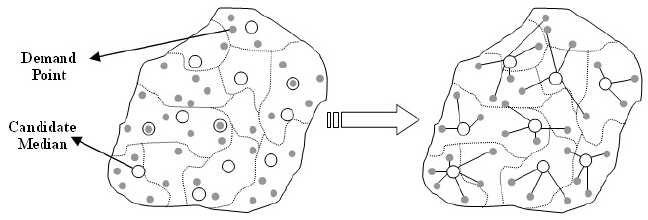
\includegraphics[width=10cm,keepaspectratio]{images/p-medians.png}
  \caption{Representação gráfica do problema das p-medianas.}
  \label{fig:p-medians}
\end{figure}

O objetivo desse trabalho é resolver o problema das p-medianas com restrições de capacidade, onde cada nó possui uma capacidade total e uma demanda por recursos pré-determinada. Ambos os problemas se encontram na categoria NP-difícil. Os detalhes técnicos e experimentais dessa implementação serão discutidos ao longo deste documento.

